\chapter{System Design and Architecture} \label{chap:chap-4}


\section{Architecture Diagram and Flow}

Gaita's architecture diagram outlines the flow of data and how various components work together to generate personalized learning pathways for users. Here is a breakdown of the system:

\begin{figure}[ht]
\begin{center}
    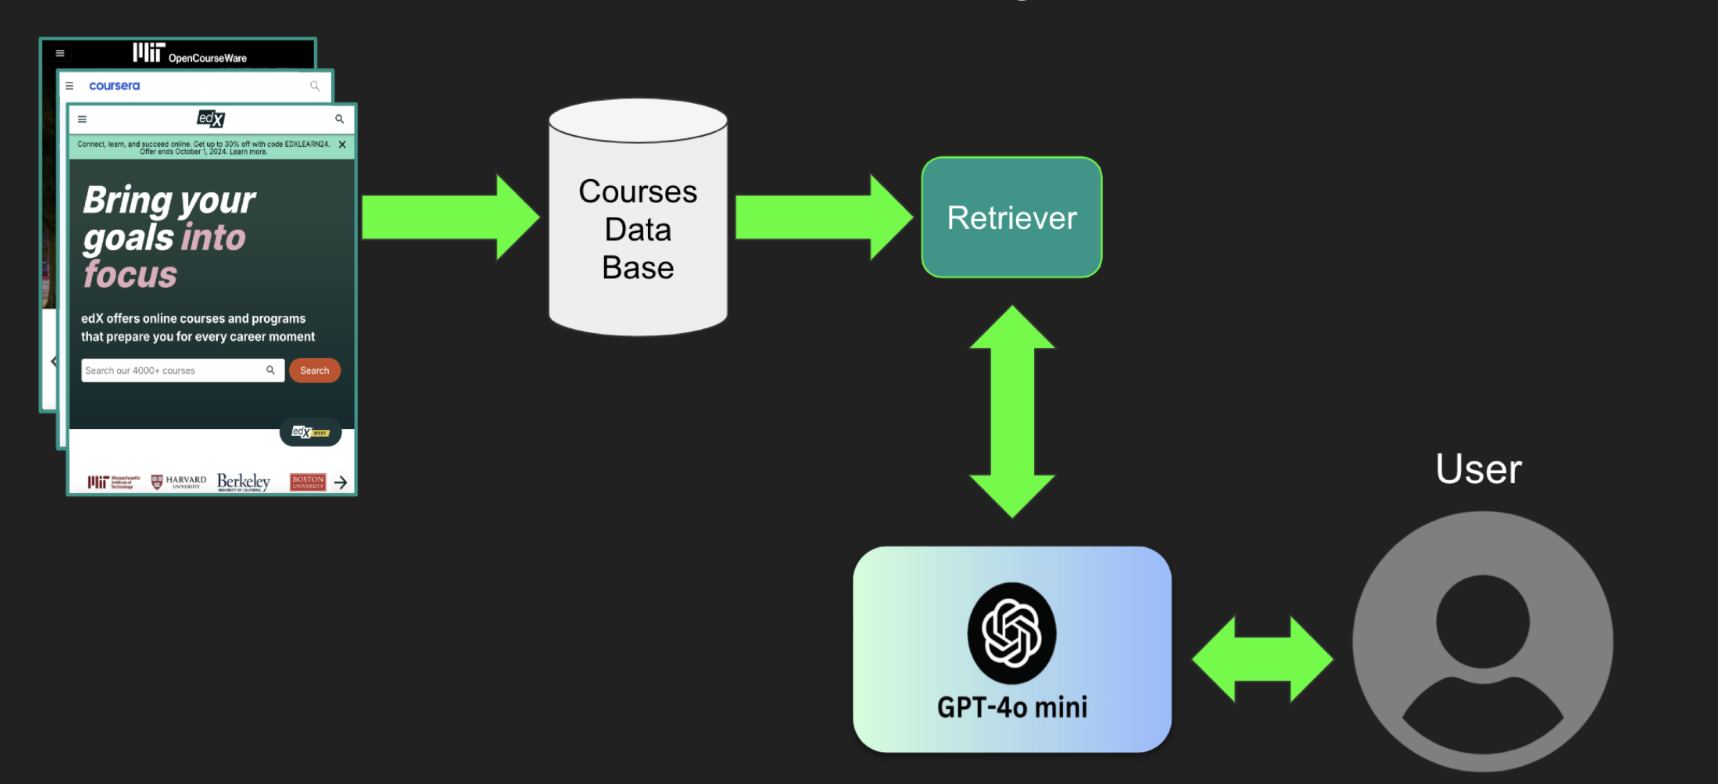
\includegraphics[width=\textwidth] {architecture_diagram.png}
    \caption{Gaita Architecture Diagram}
    \label{fig:architecture_diagram}
\end{center}
\end{figure}

\begin{enumerate}
\item \textbf{Scrape CS Courses from Coursera and MIT OCW:} Gaita collects course data from Coursera and MIT OpenCourseWare. These platforms provide high-quality Computer Science courses from leading institutions, ensuring a reliable and diverse range of learning materials.  

\item \textbf{Courses Database:} The courses from these platforms are scraped and stored in a csv file. This database contains the titles, descriptions, and URLs of over 1,200 courses.

\item \textbf{Retriever:} The "Retriever" component is responsible for retrieving the most relevant courses based on the user’s input. Using cosine similarity, the system compares the vectorized user prompt (which includes their goals and learning preferences) with the vectorized course data to identify the top 3 most relevant courses.


\item \textbf{GPT-4o Mini:} After retrieving the relevant courses, GPT-4o Mini serves the course recommendations along with descriptions of how each course fits the user’s goals and follow-up questions to gauge the user's comfort with the prerequisites for the recommended courses. 

\item \textbf{Iterative Prompting:} The system uses iterative prompting to create a personalized learning pathway. Based on the user's responses to the follow-up questions, Gaita assesses the user’s current knowledge level and recommends prerequisite courses to fill any knowledge gaps. 

\item \textbf{User Interaction:} The user interacts with Gaita through a simple and intuitive chatbot interface, where they can provide information about their background and learning goals. This interaction drives the entire recommendation pipeline, ensuring that the system continuously adapts to the learner's evolving needs.

\item \textbf{Deployed via Render:} Gaita is deployed on Render and is accessible at \url{https://gaita.onrender.com} \footnotemark[1]. \footnotetext[1] {Important: If you encounter a 502 Bad Gateway Error, this is likely because the server is currently spinning up again. Render services can sometimes take a few minutes to become fully operational, so please wait a few minutes before refreshing the page.}

\end{enumerate}


\section{Components and Technical Tools}

The following components and technical tools were used in the development of Gaita: 

\subsection{Web Crawling and Database Creation}

Web crawling is employed to collect course data from Coursera and MIT OpenCourseWare, which are both well-established platforms offering high-quality educational resources. Web crawling ensures the system has access to up-to-date content, providing a reliable external data source for generating recommendations. This data is used to create a comprehensive database of over 1,200 Computer Science courses. Our database consists of the course title, description, and URL. OpenAI’s text-embedding-3-small model was used to vectorize the course titles and descriptions in our database. 

\subsection{RAG-based Recommendation System}

The recommendation system is based on a Retrieval-Augmented Generation (RAG) approach. After receiving the user input, Cosine similarity is applied to compare the vectorized user input (i.e., their goals) with the vectorized course database. The top 3 most relevant courses are retrieved, and GPT-4o Mini is employed to serve the recommendations with descriptions of how the courses meet the user’s learning objectives.


\subsection{Turning Recommendations into Pathways}

Gaita dynamically creates a learning path through iterative prompting. After outputting course recommendations, the system generates follow-up questions to assess the learner's prior knowledge and experience. Based on the responses, prerequisite courses are recommended to fill any knowledge gaps, ensuring the learner follows a coherent learning path that aligns with their goals. This iterative process helps to dynamically create a personalized learning pathway.




